\begin{problem}{1.1}
    Let $p$ be a polynomial function on $\C$ which has no root on $S^1$. Show that the number of roots of $p(z)=0$ with $|z|<1$ is the degree of the map $\hat{p} : S^1 \to S^1$ specified by $\hat{p}(z)=p(z) / |p(z)|$.
\end{problem}

\begin{solution}
    Let $\{\xi_i\}^n_{i=1}$ be the set of roots of $p$ with $|\xi_i|<1$, and let $\{\xi_i'\}^m_{i=1}$ be the set of roots of $p$ with $|\xi_i'|>1$. (No other roots exist since $p$ has no roots on $S^1$) Then we can write
    \[p(z) = c (z-\xi_1)\cdots (z-\xi_n)(z-\xi_1')\cdots (z-\xi_m')\]
    Now consider the homotopy $H : S^1\times [0,1] \to S^1$ given by the formula
    \[H(z, t) = \frac{c(z-t\xi_1)\cdots (z-t\xi_n)(tz-\xi'_1)\cdots (tz-\xi'_m)}
{|c(z-t\xi_1)\cdots (z-t\xi_n)(tz-\xi'_1)\cdots (tz-\xi'_m)|}. 
    \]
    This is a continuous homotopy since $|t\xi_i|<1$ and $|\xi_i'/t|>1$ for $t>0$. Then, $H(z,1)=\hat{p}(z)=p(z)/|p(z)|$, but notice that $H(z,0)=(c/|c|)z^n$, a map of degree $n$. So $\hat{p}$ also has degree $n$, since the two maps are homotopic by $H$. $n$ is exactly the number of roots of $p(z)$ with magnitude $|z|<1$, so we are done.
\end{solution}

\begin{problem}{1.2}
    Show that any map $f : S^1 \to S^1$ such that $\deg(f)\neq 1$ has a fixed point.
\end{problem}

\begin{solution}
    We'll use a classic technique of proving fixed point theorems in algebraic topology, namely we assume it has no fixed points, and use this to construct some impossible topological map. 

    So suppose for the sake of contradiction that $f$ has no fixed points. Then we can build a homotopy $H: S^1\times I \to S^1$ between $f(z)$ and $z$ given by
    \[H(z,t) = \frac{tf(z)-(1-t)z}{|tf(z)-(1-t)z|}.\]
    The homotopy is continuous, since the only time $|tf(z)-(1-t)z|=0$ is if the line connecting $f(z)$ and $-z$ crosses the origin, i.e. $f(z)=z$. This satisfies $H(z,1) = f(z)$ and $H(z,0)=z$. So the degree of $f$ should be the same as the degree of $z$, which is $1$, a contradiction since we assumed $\deg(f)\neq 1$.

    This result can be generalized without that much extra work:
    \begin{claim}
        Suppose $f,g : S^1 \to S^1$ are two maps of different degree. Then we must have some $z\in S^1$ with $f(z)=g(z)$.
    \end{claim}
\end{solution}

\begin{problem}{1.3}
    Let $G$ be a topological group and take its identity element $e$ as its base-point. Define the pointwise product of loops $\alpha$ and $\beta$ by $(\alpha\beta)(t)=\alpha(t)\beta(t)$. Prove that $\alpha\beta$ is equivalent to the composition of paths $\beta\cdot \alpha$. Deduce that $\pi_1(G,e)$ is abelian.
\end{problem}

\begin{solution}
    There are two ways of solving this problem, one is a standard application of the Eckmann–Hilton argument, and the other is an application of ``abstract nonsense'' due to Grothendieck. The abstract nonsense proof uses parts of category theory we haven't discussed yet, so it's definitely not the expected proof for this problem, but it's very elegant nonetheless, so I will include part of it here after the main solution.

    The key insight here is to notice that, abstractly, we have two operations on the space of loops in $G$ up to homotopy, one taking two loops to their composition, and the other taking two loops to their pointwise product. Let's call these $*$ and $\cdot$ respectively. 
    We've shown that $*$ is well-defined on homotopy classes on $G$, this is why we can even define a fundamental group in the first place. But we can also show that $\cdot$ is well-defined on homotopy classes on paths.

    \begin{claim}
        The pointwise product $\cdot$ is a well-defined operation on $\pi_1(G, e)$. (\emph{This is not technically necessary depending on how you do the proof.})
    \end{claim}

    \begin{proof}
        Note that if $\alpha \simeq \beta : [0,1] \to G$ are loops at $e$, then $\alpha\cdot \omega \simeq \beta\cdot \omega$ for any loop $\omega : [0,1] \to G$ at $e$. This is because if $H: [0,1]\times [0,1] \to G$ is a homotopy between $\alpha$ and $\beta$, then $H\cdot \omega$ is a homotopy from $\alpha\cdot \omega$ to $\beta\cdot \omega$. We can do the same thing for $\omega\cdot \alpha$ and $\omega\cdot \beta$.
    \end{proof}

    Next, let's identify the identity elements for both operations. Recall that the identity for $*$ is the constant loop $c_e$. This turns out to be the identity element for $\cdot$ as well, since $(\alpha \cdot c_e)(t) = \alpha(t)\cdot e = \alpha(t)$. We can use this fact to prove the claim; note that for loops $\alpha,\beta$, we have
    \[
        \begin{aligned}
            (\alpha\cdot \beta)(t) = ((\alpha * c_e) \cdot (c_e * \beta))(t) &= \begin{cases}\alpha(2t)\cdot e&0\leq t<1/2,\\ e\cdot \beta(2t-1)&1/2\leq t\leq 1\end{cases}\\
            &=     \begin{cases}
                                                                        \alpha(2t)&0\leq t<1/2,\\
                                                                    \beta(2t-1)& 1/2\leq t\leq 1\end{cases} = (\alpha * \beta)(t).
        \end{aligned}
    \]
    Thus, we have $\alpha \cdot \beta = \alpha * \beta$. Similarly, we can show that
    \[\alpha * \beta = \alpha\cdot \beta = (c_e * \alpha) \cdot (\beta * c_e) = (1\cdot \beta) * (\alpha \cdot 1) = \beta * \alpha.\]
    (We might need to justify these steps with a homotopy like when we proved that $\alpha \cdot \beta = \alpha * \beta$.) Once we have these explicit homotopies, this proves that $\pi_1(G, e)$ is abelian.
    
    More generally, this ``trick'' works for any two unital operations $\otimes, \times$ satisfying:
    \[
        (a\otimes b)\times (c\otimes d) = (a\times c)\otimes (b\times d),
    \]
    we can conclude that they are the same operation, and commutative. You don't actually have to do all of this work, you can prove this by just building explicit homotopies from $\alpha * \beta$ to $\alpha \cdot \beta$ and $\alpha * \beta$ to $\beta \cdot \alpha$. This is pretty much equivalent to the approach here, however if you view things more abstractly involving the two operations, it becomes easier to generalize.

    A more general, and often more useful way to see this same result is an argument due to Grothendieck, which we need some category theory to properly state.

    \begin{definition}
        Let $\CC$ be a category with (finite) products. By this definition, it should have some \emph{terminal object}, which we call $1\in \CC$. (Recall that a terminal object is some object $1$ that has a morphism $X \to 1$ to any $X\in \CC$.) A \emph{group object} in $\CC$ is an object $G$ of $\CC$ together with morphisms
        \begin{enumerate}[(i)]
            \item $\mu : G\times  G \to G$, (\emph{multiplication})
            \item $e : 1 \to G$, (\emph{identity})
            \item $\iota : G \to G$, (\emph{inversion})
        \end{enumerate}
        such that the following equalities hold:
        \begin{enumerate}[(i)]
            \item $\mu(\mu\times \textrm{id}_G) = \mu(\textrm{id}_G \times \mu)$. 
            \item $\mu(e\times \textrm{id}_G) = \pi_G$ and $\mu(\textrm{id}_G \times e) = \pi_G$ where $\pi_G : 1\times G \to G$ or $G\times 1\to G$ is the projection.
            \item $\iota$ is a two-sided inverse for $m$, i.e. letting $\Delta : G \to G\times G$ be the diagonal map and $e_G : G\to G$ the terminal map sending $G \to 1$ composed with $e$, we have $m(\textrm{id}_G \times \iota)\circ \Delta = m(\iota \circ \textrm{id}_G)\circ \Delta = e_G$. 
        \end{enumerate}
    \end{definition}
    This is a fairly abstract definition, notice that we only used properties of canonical maps to construct a group object, we don't even require that the ``groups'' we construct contain elements at all. Our regular notion of a group is simply a group object in $\textbf{Set}$, and a group object in $\textbf{Grp}$ is an \emph{abelian group}. (Check this fact!) Similarly, a group object in the category of smooth manifolds is a \emph{Lie group}, a group object in the category of topological spaces is a topological group, and similarly for other categories. These group objects also behave very well with functors, as we can see in the following proposition: 

    \begin{claim}
        Let $\CC, \mathscr{D}$ be categories with finite products, and $F : \CC \to \mathscr{D}$ be a functor preserving products. Then $F$ sends group objects to group objects.
    \end{claim}
    \begin{proof}
        Exercise; this is fairly direct using the definition of a group object and definition of a functor.
    \end{proof}
    Now with this background, we have a one-line solution to the problem we're trying to solve:

    \begin{center}
        \emph{$\pi_1 : \mathbf{pcTop_*} \to \mathbf{Grp}$ preserves products, so it sends topological groups to abelian groups.}
    \end{center}

    (Here $\mathbf{pcTop_*}$ is the category of path-connected topological spaces with basepoints, feel free to think of $\mathbf{Top}$ if it's easier, the general argument is the same.)

    \medskip
    If you haven't seen why $\pi_1(X\times Y)\cong \pi_1(X)\times \pi_1(Y)$, this is a good thing to check for yourself. Otherwise, assuming you also had all the category theory already developed, the answer becomes quite immediate, otherwise it takes a bit more work. Later on when we get to higher homotopy groups and cohomology, we might introduce the notion of an $H$-group, which is defined:

    \begin{definition}
        An \emph{$H$-group} is a group object in the homotopy category $\textbf{hTop}$. This is sort of like a ``homotopy theoretic'' version of a topological group, and works more naturally in a homotopy theory setting. An \emph{$H$-space} relaxes the assumptions even more by not requiring inversion, and this definition is also common.
    \end{definition}

    Immediately, by our abstract nonsense argument we can conclude that the fundamental group of any $H$-group is abelian, and this is a useful fact in homotopy theory. This is because the \emph{loop space} $\Omega X$ of any space $X$ can be given an $H$-group structure by something resembling loop composition. In particular, we have
    \[\pi_n(X) = \pi_1(\Omega^{n-1} X),\]
    so we've just concluded that $\pi_n$ are abelian for all $n\geq 2$!
\end{solution}

\begin{problem}{2.1}
    Compute the fundamental group of the two-holed torus (the compact surface of genus $2$ obtained by sewing together two tori along the boundaries of an open disk removed from each).
\end{problem}

Recall that the fundamental group of the torus is $\pi_1(S^1\times S^1) = \pi_1(S^1)\times \pi_1(S^1) = \Z\oplus \Z$, with one generator going around the torus horizontally, and the other going around vertically. We can cut a small simply connected disk in each torus and glue them together along the boundary of this disk. Then we let $U = T^2-\Delta$ be the first punctured torus, and $V = T^2-\Delta$ be the second punctured torus embedded in the two-holed torus.

\[
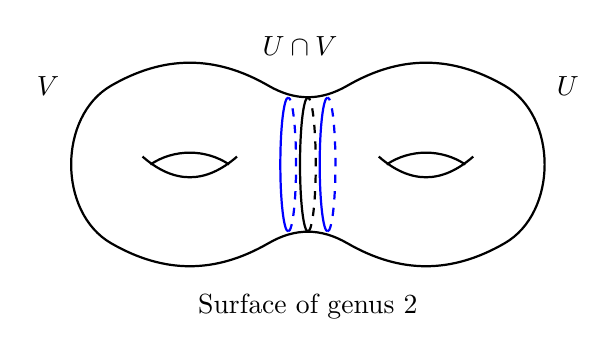
\begin{tikzpicture}
\draw[smooth, thick] (0,1) to[out=30,in=150] (2,1) to[out=-30,in=210] (3,1) to[out=30,in=150] (5,1) to[out=-30,in=30] (5,-1) to[out=210,in=-30] (3,-1) to[out=150,in=30] (2,-1) to[out=210,in=-30] (0,-1) to[out=150,in=-150] (0,1);
\draw[smooth, thick] (0.4,0.1) .. controls (0.8,-0.25) and (1.2,-0.25) .. (1.6,0.1);
\draw[smooth, thick] (0.5,0) .. controls (0.8,0.2) and (1.2,0.2) .. (1.5,0);
\draw[smooth, thick] (3.4,0.1) .. controls (3.8,-0.25) and (4.2,-0.25) .. (4.6,0.1);
\draw[smooth, thick] (3.5,0) .. controls (3.8,0.2) and (4.2,0.2) .. (4.5,0);

\draw[thick] (2.5,-0.85) arc(270:90:0.1 and 0.85);
\draw[dashed, thick] (2.5,-0.85) arc(270:450:0.1 and 0.85);

\draw[blue, thick] (2.75,-0.85) arc(270:90:0.1 and 0.85);
\draw[blue, dashed, thick] (2.75,-0.85) arc(270:450:0.1 and 0.85);

\draw[blue, thick] (2.25,-0.85) arc(270:90:0.1 and 0.85);
\draw[blue, dashed, thick] (2.25,-0.85) arc(270:450:0.1 and 0.85);
 \node at (5.8,1) {$U$};
 \node at (-0.8,1) {$V$};
 \node at (2.4,1.5) {$U\cap V$};
    \node at (2.5,-1.8) {Surface of genus $2$};
\end{tikzpicture}
\]

These are both path-connected open sets with path-connected intersection, so we can apply the Seifert-Van Kampen theorem. Assuming some basepoint, we need to figure out the homotopy groups $\pi_1(U\cap V)$, $\pi_1(U)$, $\pi_1(V)$, as well as the homomorphisms $\pi_1(U \to U\cap V)$, and $\pi_1(V \to U\cap V)$. For the first part, it's clear that $U\cap V$ is an open cylinder so $U\cap V\simeq S^1\times (0,1)\simeq S^1$ and so $\pi_1(U\cap V)\cong \Z$.

The other open sets $U,V$ are both homeomorphic to the punctured torus $S^1\times S^1-\{p\}$. It's best to understand this space by looking at the parametrization of $S^1\times S^1$ as a quotient of a square with sides idenfitified:

\[
    \begin{tikzpicture}
        \begin{scope}[thick, xshift=3cm]
            \draw[red, postaction={decorate}, decoration={
                markings,
                mark=at position 0.50 with {\arrow{latex}}}
            ] (0,0) -- (2,0) {};
            \draw[red, postaction={decorate}, decoration={
                markings,
                mark=at position 0.50 with {\arrow{latex}}}
            ] (0,2) -- (2,2) {};

            \draw[blue, postaction={decorate}, decoration={
                markings,
                mark=at position 0.50 with {\arrow{latex}}}
            ] (0,0) -- (0,2) {};
            \draw[blue, postaction={decorate}, decoration={
                markings,
                mark=at position 0.50 with {\arrow{latex}}}
            ] (2,0) -- (2,2) {};
            \node at (1,-0.5) {Wedge product $S^1\vee S^1$};
            \node at (2.6, 1) {$a^{-1}$};
            \node at (-0.4, 1) {$a$};
            \node at (1, 2.4) {$b$};
            \node at (1, 0.4) {$b^{-1}$};
        \end{scope}
        \draw [-latex,thick] (0,1) -- node[above] {$\sim$} (2,1);
        \begin{scope}[thick, xshift=-3cm]
            \draw[fill=white!95!black] (0,0) -- (2,0) -- (2,2) -- (0,2) -- cycle;
            \draw[black, dashed, fill = white] (1.0,1.0) ellipse (0.2 and 0.2);

            \draw[red, postaction={decorate}, decoration={
                markings,
                mark=at position 0.50 with {\arrow{latex}}}
            ] (0,0) -- (2,0) {};
            \draw[red, postaction={decorate}, decoration={
                markings,
                mark=at position 0.50 with {\arrow{latex}}}
            ] (0,2) -- (2,2) {};

            \draw[blue, postaction={decorate}, decoration={
                markings,
                mark=at position 0.50 with {\arrow{latex}}}
            ] (0,0) -- (0,2) {};
            \draw[blue, postaction={decorate}, decoration={
                markings,
                mark=at position 0.50 with {\arrow{latex}}}
            ] (2,0) -- (2,2) {};
            \node at (1,-0.5) {Punctured torus $S^1\times S^1 - \{p\}$};
        \end{scope}
    \end{tikzpicture}
\]
This punctured torus thus deformation retracts onto the wedge product $S^1\vee S^1$, so $\pi_1(U), \pi_1(V) \cong \Z a * \Z b$. All we have left to do is to understand the maps $\pi_1(U\cap V) \to \pi_1(U)$. Under the above parametrization, a generator of $U\cap V$ would get mapped to a loop going once around the center hole of the square, and in the deformation retract, this loop would get mapped to $aba^{-1}b^{-1} \in \Z a *\Z b$. This can be seen by tracing its path along the boundary and seeing what happens after the quotient identification.

Thus, we have the following diagrams of fundamental groups:

\[
\begin{tikzcd}
{\pi_1(U\cap V)} & {\pi_1(U)} \\
{\pi_1(V)}
\arrow["{(i_V)_*}"', from=1-1, to=2-1]
\arrow["{(i_U)_*}", from=1-1, to=1-2]
\end{tikzcd}\quad\implies\quad
\begin{tikzcd}
	\Z & {\Z a*\Z b} \\
	{\Z a'*\Z b'}
	\arrow["{aba^{-1}b^{-1}}", from=1-1, to=1-2]
	\arrow["{a'b'(a')^{-1}(b')^{-1}}"', from=1-1, to=2-1]
\end{tikzcd}
\]
The Seifert-Van Kampen theorem tells us that the pushout of this diagram should be the fundamental group of the two-holed torus. But the pushout in the category of groups is the ``amalgamated free product'', which has the form:
\[\begin{aligned}\pi_1(U)*_{\pi_1(U\cap V)} \pi_1(V) \cong (\Z a * \Z b) *_{\Z} (\Z c * \Z d) &\cong\frac{\Z a * \Z b * \Z a' * \Z b'}{aba^{-1}b^{-1}=a'b'(a')^{-1}(b')^{-1}}\\
&\cong \langle x, y, z, w \mid xyx^{-1}y^{-1} zwz^{-1}w^{-1}\rangle.\end{aligned}\]
This group is \emph{not} free abelian, unlike the case for the torus. The \emph{abelianization} of this group however is $\Z\oplus \Z \oplus \Z \oplus \Z$, so maybe the pattern inherited from the one-holed torus is still true in a sense. We'll learn more about this when we study homology.

\medskip
This operation of ``sewing together'' two compact surfaces along some cut out disk is called the \emph{connected sum}, and denoted $M_1 \# M_2$. This is a fundamental operation in the theory of compact surfaces, in fact we can prove:

\begin{claim}[Classification of Compact Surfaces]
    Let $M$ be a compact surface. Then $M$ is homeomorphic to exactly one of the following:
    \begin{enumerate}[(i)]
        \item $S^2$. (\emph{trivial case})
        \item $T^2 \# T^2 \# \cdots \# T^2$. (\emph{orientable, torus with $n$ holes})
        \item $\RP^2 \# \RP^2 \# \cdots \# \RP^2$. (\emph{not orientable, cannot be embedded in $\R^3$})
    \end{enumerate}
\end{claim}

If you want a slightly challenging exercise, try computing the fundamental groups of all of these surfaces; this will immediately tell us that all of these surfaces are topologically distinct.

\medskip
Getting a bit sidetracked, we could investigate the relationships between the different types of surfaces in this list. At some point, we'd stumble onto the following relation:

\begin{claim}
    We have a homeomorphism $T^2\# \RP^2 \cong \RP^2\# \RP^2 \# \RP^2$.
\end{claim}
\begin{proof}
    Draw a picture; what does it mean to take a connected sum with a torus?
\end{proof}

This turns out to be \emph{the defining algebraic relation} for compact surfaces! If we consider connected sum as a commutative operation, we form a \emph{monoid} of compact surfaces, say $\mathbf{Surf}$. With some work, we can construct an isomorphism on monoids:
\[\textbf{Surf} \cong \langle T, P \mid T\oplus P = 3P\rangle.\]
This is a complete \emph{algebraic} classification of \emph{topological} objects! Later on when we discuss the beautiful theorem of Poincare duality, this will become a natural consequence of the \emph{intersection pairing}, which allows us to associate a $\mathbb{F}_2$-bilinear form to each surface of even dimension.

\begin{problem}{2.2}
    The Klein bottle $K$ is the quotient space of $S^1\times I$ obtained by identifying $(z,0)$ with $(z^{-1},1)$ for $z\in S^1$. Compute $\pi_1(K)$.
\end{problem}

In this problem, we can go straight for the parametrization, and directly do a Seifert decomposition:

\[
    \begin{tikzpicture}
        \begin{scope}[thick, xshift=-3cm]
            \draw[fill=white!95!black] (0,0) -- (2,0) -- (2,2) -- (0,2) -- cycle;

            \draw[red, postaction={decorate}, decoration={
                markings,
                mark=at position 0.50 with {\arrow{latex}}}
            ] (0,0) -- (2,0) {};
            \draw[red, postaction={decorate}, decoration={
                markings,
                mark=at position 0.50 with {\arrow{latex}}}
            ] (0,2) -- (2,2) {};

            \draw[blue, postaction={decorate}, decoration={
                markings,
                mark=at position 0.50 with {\arrow{latex}}}
            ] (0,0) -- (0,2) {};
            \draw[blue, postaction={decorate}, decoration={
                markings,
                mark=at position 0.55 with {\arrow{latex}}}
            ] (2,2) -- (2,0) {};
            \node at (1,-0.5) {Klein bottle $K$};
        \end{scope}

        \draw [-latex,thick] (0,1) -- node[above] {$=$} (2,1);
        \begin{scope}[thick, xshift=3cm]
            \draw[fill=white!95!black] (0,0) -- (2,0) -- (2,2) -- (0,2) -- cycle;
            \draw[black, dashed, fill = white] (1.0,1.0) ellipse (0.4 and 0.4);

            \draw[red, postaction={decorate}, decoration={
                markings,
                mark=at position 0.50 with {\arrow{latex}}}
            ] (0,0) -- (2,0) {};
            \draw[red, postaction={decorate}, decoration={
                markings,
                mark=at position 0.50 with {\arrow{latex}}}
            ] (0,2) -- (2,2) {};

            \draw[blue, postaction={decorate}, decoration={
                markings,
                mark=at position 0.50 with {\arrow{latex}}}
            ] (0,0) -- (0,2) {};
            \draw[blue, postaction={decorate}, decoration={
                markings,
                mark=at position 0.55 with {\arrow{latex}}}
            ] (2,2) -- (2,0) {};
            \node at (1,-0.5) {Punctured Klein bottle $K^*$};
        \end{scope}
        \begin{scope}[thick, xshift=7cm]
            \draw[black, dashed, fill = white!95!black] (1.0,1.0) ellipse (0.7 and 0.7);
            \node at (-0.8,1) {$\bigcup$};
            \node at (1,-0.5) {Open disk $D$};
        \end{scope}
    \end{tikzpicture}
\]

The open disk is contractible, so it makes no contribution to the total space. The intersection of $D\cap K^*$ however, is homotopy equivalent to a circle so this has an effect. In fact, since we only have one nonzero term in the amalgamated free product, our total space is:
\[
    \pi_1(K) \cong \pi_1(K^*) *_{\pi_1(D\cap K^*)} \{0\}\cong \textrm{coker}(\pi_1(D\cap K^*) \to \pi_1(K^*)) \cong \frac{\pi_1(K^*)}{\textrm{Im}(\pi_1(D\cap K^*))}
\]
Notice that by the same argument that we did for the two-holed torus, we can see that $K^*$ is homotopy equivalent to the wedge product $S_1\vee S_1$:

\[
    \begin{tikzpicture}
        \begin{scope}[thick, xshift=3cm]
            \draw[red, postaction={decorate}, decoration={
                markings,
                mark=at position 0.50 with {\arrow{latex}}}
            ] (0,0) -- (2,0) {};
            \draw[red, postaction={decorate}, decoration={
                markings,
                mark=at position 0.50 with {\arrow{latex}}}
            ] (0,2) -- (2,2) {};

            \draw[blue, postaction={decorate}, decoration={
                markings,
                mark=at position 0.50 with {\arrow{latex}}}
            ] (0,0) -- (0,2) {};
            \draw[blue, postaction={decorate}, decoration={
                markings,
                mark=at position 0.55 with {\arrow{latex}}}
            ] (2,2) -- (2,0) {};
            \node at (1,-0.5) {Wedge product $S^1\vee S^1$};
            \node at (2.6, 1) {$a$};
            \node at (-0.4, 1) {$a$};
            \node at (1, 2.4) {$b$};
            \node at (1, 0.4) {$b^{-1}$};
        \end{scope}
        \draw [-latex,thick] (0,1) -- node[above] {$\sim$} (2,1);
        \begin{scope}[thick, xshift=-3cm]
            \draw[fill=white!95!black] (0,0) -- (2,0) -- (2,2) -- (0,2) -- cycle;
            \draw[black, dashed, fill = white] (1.0,1.0) ellipse (0.4 and 0.4);

            \draw[red, postaction={decorate}, decoration={
                markings,
                mark=at position 0.50 with {\arrow{latex}}}
            ] (0,0) -- (2,0) {};
            \draw[red, postaction={decorate}, decoration={
                markings,
                mark=at position 0.50 with {\arrow{latex}}}
            ] (0,2) -- (2,2) {};

            \draw[blue, postaction={decorate}, decoration={
                markings,
                mark=at position 0.50 with {\arrow{latex}}}
            ] (0,0) -- (0,2) {};
            \draw[blue, postaction={decorate}, decoration={
                markings,
                mark=at position 0.55 with {\arrow{latex}}}
            ] (2,2) -- (2,0) {};
            \node at (1,-0.5) {Punctured Klein bottle $K^*$};
        \end{scope}
    \end{tikzpicture}
\]
Then we can conclude by seeing what happens to the loop around the hole that
\[\pi_1(K) \cong \Z a * \Z b *_{\Z} \{0\} \cong \frac{\Z a * \Z b}{abab^{-1}} \cong \langle a, b \mid abab^{-1}\rangle.\]
This group is also not free abelian, however it's abelianization is $\Z\oplus \Z /2$, we'll see this come up later when we calculate homology groups.

\medskip
In the last problem, we discussed the classification of compact surfaces. Which of the surfaces on the list is $K$ homeomorphic to?

\begin{problem}{2.3} Let $X = \{(p,q)\; : \; p\neq -q\}\subset S^n\times S^n$. Define a map $f : S^n \to X$ by $f(p)=(p,p)$. Prove that $f$ is a homotopy equivalence.
\end{problem}

\begin{solution}
    Consider the map $g : X \to S^n$ given by $g(p,q) = p$. This is a left inverse for $f$, since $g(f(p)) = g(p,p) = p$ so $g\circ f = \textrm{id}_{S^n}$. It's not a right inverse for $f$, but is a homotopy right inverse, which is what we'll check. Consider the homotopy $H: X\times [0,1] \to X$ given by:
    \[
        H((p,q), t) = (p, g_{p,q}(t)),\quad\textrm{where}\quad g_{p,q}(t)=\frac{(1-t)p+tq}{|(1-t)p+tq|}.
    \]
    This $g_{p,q}$ is the \emph{geodesic path} from $p$ to $q$, and well-defined since $p\neq -q$. (Otherwise there would be two equal-length paths from $p$ to $q$.)
    \[
        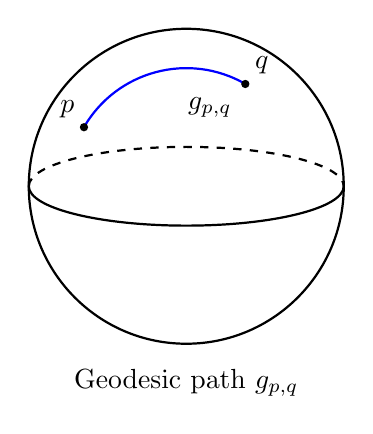
\begin{tikzpicture}
            % Draw the circle representing the sphere
            \draw[thick] (0,0) circle (2cm);
            
            \node at (0.3,1.0) {$g_{p,q}$};
            % Draw the geodesic as an arc
            \draw[blue, thick] (150:1.5cm) arc (150:60:1.5cm);
    
            \draw[thick] (-2,0) arc (180:360:2cm and 0.5cm);
            \draw[dashed, thick] (-2,0) arc (180:360:2cm and -0.5cm);
            
            % Mark points p and q
            \fill (150:1.5cm) circle (1.5pt) node[anchor=south east] {$p$};
            \fill (60:1.5cm) circle (1.5pt) node[anchor=south west] {$q$};
            \node at (0,-2.5) {Geodesic path $g_{p,q}$};
        \end{tikzpicture}
    \]
    Then $H((p,q), 1) = (p,q)=\textrm{id}_X$, and $H((p,q),0)=f(g(p,q))$ so $f\simeq g$.

    \medskip
    This map $g : X \to S^n$ gives $X$ the structure of a \emph{fiber bundle} over $S^n$. Note that the fibers of this bundle look like $g^{-1}(p) = S^n-\{-p\}$, which is homeomorphic to a hyperplane $\R^n$. So this is actually a \emph{plane bundle}. This is hard to visualize when $n\geq 1$, however when $n=1$, this admits a very satisfying picture:
    \[
        \begin{asypicture}{name=torus}
            import graph3;
           
            size(200,0);
            currentprojection=orthographic(4,0,2);
           
            //inner radius
            real R=2;
            //outer radius
            real a=0.75;
           
            //surface:
            triple f(pair t) {
              return ((R+a*cos(t.y))*cos(t.x),(R+a*cos(t.y))*sin(t.x),a*sin(t.y));
            }
           
            real p = 2;
            real q = 2;

            //path:
            real x(real t) {return cos(p*t)*(R + a*cos(q*t));}
            real y(real t) {return sin(p*t)*(R + a*cos(q*t));}
            real z(real t) {return a*sin(q*t);}
           
            real xa(real t) {return -cos(p*t)*(R + a*cos(q*t));}
            real ya(real t) {return sin(p*t)*(R + a*cos(q*t));}
            real za(real t) {return -a*sin(q*t);}

            pen p=blue+opacity(0.33);
            // make surface and path
            surface s=surface(f,(0,0),(2pi,2pi),8,8,Spline);
            path3 q=graph(x,y,z,0,2*pi,operator ..);
            path3 qa = graph(xa,ya,za, 0, 2*pi, operator..);
           
            // draw surface and path
            draw(s,surfacepen=material(diffusepen=white+opacity(0.70), emissivepen=gray));
            draw(q, p=1pt+gray);
            draw(qa, p=2pt+blue);
        \end{asypicture}
    \]
    \[
        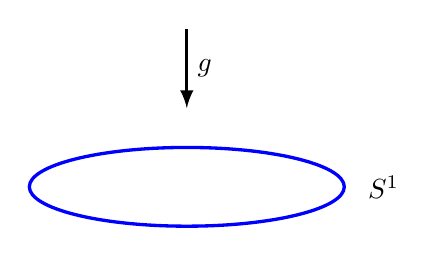
\begin{tikzpicture}
            \draw[black, very thick, -latex] (0,0) -- node[right] {$g$} (0,-1);
            \draw[blue, very thick] (0,-2) ellipse (2cm and 0.5cm);
            \node at (2.5,-2) {$S^1$};
        \end{tikzpicture}
    \]

    Here the gray line is the curve $(p,-p)$ cut out of the torus, and the blue line is the image of $f$, i.e. the curve $(p,p)$. You can imagine the homotopy as retracting the torus away from the cutout curve towards the blue curve along geodesic curves on each vertical circular slice of the torus. If we view this as a $(S^1-\{p\})\cong \R$-bundle, what does this bundle look like?
\end{solution}

\begin{problem}{2.4}
    Let $\CC$ be a category that has all coproducts and coequalizers. Prove that $\CC$ is cocomplete (has all colimits). Deduce formally, by use of opposite categories, that a category that has all products and equalizers is complete.
\end{problem}

\begin{solution}
    Let's first do an example to get an intuition for how to build colimits out of coproducts and coequalizers. We'll work in the category of sets to make things more intuitive.

    \begin{example}
        Let $A, B, C$ be sets and $f : B \to A$ and $g : B \to C$ be functions. The \emph{pushout} of this diagram in $\textbf{Set}$ is the colimit of the diagram $A \leftarrow B \rightarrow C$, i.e. 
        % https://q.uiver.app/#q=WzAsNCxbMCwwLCJCIl0sWzEsMCwiQSJdLFswLDEsIkMiXSxbMSwxLCJBXFxzcWN1cF9CQyJdLFswLDEsImYiXSxbMCwyLCJnIiwyXSxbMiwzXSxbMSwzXV0=
        \[\begin{tikzcd}
	        B & A \\
	        C & {A\sqcup_BC}
	        \arrow["f", from=1-1, to=1-2]
	        \arrow["g"', from=1-1, to=2-1]
	        \arrow[from=2-1, to=2-2]
	        \arrow[from=1-2, to=2-2]
        \end{tikzcd}\quad \implies\quad A\sqcup_B C = \frac{A\sqcup C}{f(b)\sim g(b),\; \forall b\in B}. \]
        In other words, we ``glue'' $A$ and $C$ together along $B$ by the maps $f$, $g$.
    \end{example}

    \begin{solution}
        We can express this construction as a coequalizer/coproduct of spaces and maps in $\textbf{Set}$. Particularly, consider the coequalizer 
        % https://q.uiver.app/#q=WzAsMyxbMCwwLCJCIl0sWzEsMCwiQVxcc3FjdXAgQyJdLFsyLDAsIlxcQ29lcShcXGlvdGFfQVxcY2lyYyBmLCBcXGlvdGFfQ1xcY2lyYyBnKSJdLFswLDEsIlxcaW90YV9BXFxjaXJjIGYiLDAseyJvZmZzZXQiOi0xfV0sWzAsMSwiXFxpb3RhX0NcXGNpcmMgZyIsMix7Im9mZnNldCI6MX1dLFsxLDJdXQ==
        \[\begin{tikzcd}
	        B && {A\sqcup C} & {\Coeq(\iota_A\circ f, \iota_C\circ g)}
	        \arrow["{\iota_A\circ f}", shift left, from=1-1, to=1-3]
	        \arrow["{\iota_C\circ g}"', shift right, from=1-1, to=1-3]
	        \arrow[from=1-3, to=1-4]
        \end{tikzcd},\]
        where $\iota_A : A \to A\sqcup C$ and $\iota_C : C \to A\sqcup C$ are the canonical inclusions. By abuse of notation we could also just write this as 
        \[\begin{tikzcd}
	        B & {A\sqcup C} & {\Coeq(f, g)}
	        \arrow["{f}", shift left, from=1-1, to=1-2]
	        \arrow["{g}"', shift right, from=1-1, to=1-2]
	        \arrow[from=1-2, to=1-3]
        \end{tikzcd},\]
        but we should be careful to remember that there should be explicit inclusion maps to be safe when working in a general category. This coequalizer then has the exact same form as the pushout from before, its the quotient
        \[\Coeq(f,g) = \frac{A\sqcup C}{f(b) \sim g(b),\; \forall b\in B} = A\sqcup_B C.\]
        But we might have a hard time generalizing this approach. 
        Let's express it as a different coequalizer which might be easier to apply other colimits. Consider the pair of maps:
        % https://q.uiver.app/#q=WzAsMixbMCwwLCJCXFxzcWN1cCBCIl0sWzIsMCwiQVxcc3FjdXAgQ1xcc3FjdXAgQiJdLFswLDEsIkwiLDAseyJvZmZzZXQiOi0xfV0sWzAsMSwiSyIsMix7Im9mZnNldCI6MX1dXQ==
        \[\begin{tikzcd}
	        {B\sqcup B} && {A\sqcup C\sqcup B}
	        \arrow["L", shift left, from=1-1, to=1-3]
	        \arrow["K"', shift right, from=1-1, to=1-3]
        \end{tikzcd}\]
        defined in the following way: We let (with some abuse of notation) $L(b) = L(b') = b$, i.e. it sends any $b$ in $B\sqcup B$ (either the first or second component) to the $B$ in $A\sqcup C\sqcup B$. Then, let $K(b)=f(b)\in A$ for the first $B$, and $K(b')=g(b')\in B$ for the second $B$. (This can be expressed more rigorously with explicit inclusion maps, hence my warning earlier.)
        Then, the coequalizer of this diagram should be the quotient:
        \[
            \begin{aligned}
                \Coeq(L, K) = \frac{A\sqcup B\sqcup C}{K(b)\sim L(b), K(b')\sim L(b'),\; \forall b,b'\in B} &= \frac{A\sqcup B\sqcup C}{f(b)\sim b, g(b)\sim b,\; \forall b\in B}\\ 
                &= \frac{A\sqcup C}{f(b)\sim g(b),\;\forall b\in B} = A\sqcup_B C.
            \end{aligned}
        \]
        Notice that we have one term in the source coproduct for every ``base'' of a map in a diagram, and one term in the target coproduct for every object in the diagram. Then, one of our maps acts like an identity, and the other sends all the ``base'' terms to their target.
    \end{solution}

    Let's use this approach to do this in a general category, so suppose we have a category $\CC$. Remember that a diagram in $\CC$ is a functor from some (small) index/diagram category $I$ to $\CC$, so let's say $F : I \to \CC$.
    Just like in our example, our base coproduct is: 
    \[
        B_F = \coprod_{f\in \Hom_I(i, j)} F(i),
    \]
    i.e. the coproduct of all source objects for all arrows in the diagram. Then the target coproduct is:
    \[
        T_F = \coprod_{k\in I} F(k),
    \]
    i.e. the coproduct of every object in the diagram. Let's define the function $L_F : B_F \to T_F$ by setting $L_F(x) = x\in F(i)$ where $x\in F(i)$, the component corresponding to $f\in \Hom_I(i,j)$. Similarly, we let $K_F : B_F \to T_F$ be the map defined by $K_F(x) = f(x)\in F(j)$, where $x\in F(i)$, the component corresponding to $f\in \Hom_I(i,j)$. So we get a coequalizer:

    \[\begin{tikzcd}
	    B_F && T_F & \Coeq(L_F, K_F)
	    \arrow["L_F", shift left, from=1-1, to=1-3]
	    \arrow["K_F"', shift right, from=1-1, to=1-3]
	    \arrow["", shift right, from=1-3, to=1-4]
    \end{tikzcd}\]
    Let's prove that $\Coeq(L_F, K_F)\cong \colim_{i\in I} F(i)$. To do this, let $\iota_f : F(i) \to B_F$ be the inclusion for some $f\in \Hom_I(i,j)$, and let $i_k: F(k) \to T_F$ be the inclusion for some $k\in I$.

    \medskip
    Since colimits are unique up to isomorphism, we just need to check that $\Coeq(L_F, K_F)$ satisfies the universal property of a colimit. 
    
    \begin{part}{Step 1}
        We want a map $\iota_i : F(i) \to \Coeq(L_F, K_F)$ for all $i\in I$.
    \end{part}
    \begin{solution}

    This isn't too bad, given some $F(i)$, we can naturally map it into $T_F$ (since $T_F$ is just a coproduct of all $F(i)$) and then compose with the map $T_F \to \Coeq(L_F, K_F)$.
    % https://q.uiver.app/#q=WzAsNCxbMiwwLCJUX0YiXSxbMCwwLCJCX0YiXSxbMywwLCJcXENvZXEoTF9GLCBLX0YpIl0sWzIsMSwiRihpKSJdLFsxLDAsIiIsMCx7Im9mZnNldCI6MX1dLFsxLDAsIiIsMix7Im9mZnNldCI6LTF9XSxbMCwyXSxbMywwXSxbMywyLCJcXGlvdGFfaSIsMix7ImNvbG91ciI6WzM1OSwxMDAsNjBdLCJzdHlsZSI6eyJib2R5Ijp7Im5hbWUiOiJkYXNoZWQifX19LFszNTksMTAwLDYwLDFdXV0=
    \[\begin{tikzcd}
	    {B_F} && {T_F} & {\Coeq(L_F, K_F)} \\
	    && {F(i)}
	    \arrow[shift right, from=1-1, to=1-3]
	    \arrow[shift left, from=1-1, to=1-3]
	    \arrow[from=1-3, to=1-4]
	    \arrow[from=2-3, to=1-3]
	    \arrow["{\iota_i}"', color=red, dashed, from=2-3, to=1-4]
    \end{tikzcd}\]
    Visually, our desired map is the red map in the above diagram.
    \end{solution}
    
    \begin{part}{Step 2}
        These $\iota_i$ should commute with the diagram, i.e. if $f : i \to j$ is an arrow in the diagram, we should have $\iota_j\circ F(f) = \iota_i$.
    \end{part}
    \begin{solution}

    Here we can draw a slightly more complex diagram using the definition of the two maps in our coequalizer.
    % https://q.uiver.app/#q=WzAsNyxbMiwxLCJUX0YiXSxbMCwxLCJCX0YiXSxbMywxLCJcXENvZXEoTF9GLCBLX0YpIl0sWzIsMiwiRihpKSJdLFswLDIsIkYoaSkiXSxbMCwwLCJGKGkpIl0sWzIsMCwiRihqKSJdLFsxLDAsIkxfRiIsMix7Im9mZnNldCI6MX1dLFsxLDAsIktfRiIsMCx7Im9mZnNldCI6LTF9XSxbMCwyXSxbMywwXSxbMywyLCJcXGlvdGFfaSIsMl0sWzQsMV0sWzQsMywiXFx0ZXh0cm17aWR9IiwyXSxbNSw2LCJGKGYpIl0sWzUsMV0sWzYsMF0sWzYsMiwiXFxpb3RhX2oiXV0=
    \[\begin{tikzcd}
	    {F(i)} && {F(j)} \\
	    {B_F} && {T_F} & {\Coeq(L_F, K_F)} \\
	    {F(i)} && {F(i)}
	    \arrow["{L_F}"', shift right, from=2-1, to=2-3]
	    \arrow["{K_F}", shift left, from=2-1, to=2-3]
	    \arrow[from=2-3, to=2-4]
	    \arrow[from=3-3, to=2-3]
	    \arrow["{\iota_i}"', from=3-3, to=2-4]
	    \arrow[from=3-1, to=2-1]
	    \arrow["{\textrm{id}}"', from=3-1, to=3-3]
	    \arrow["{F(f)}", from=1-1, to=1-3]
	    \arrow[from=1-1, to=2-1]
	    \arrow[from=1-3, to=2-3]
	    \arrow["{\iota_j}", from=1-3, to=2-4]
    \end{tikzcd}\]

    By commutation and the \emph{universal property of the coequalizer}, tracing along the top should be the same as tracing along the bottom, since these maps will be equal in the coequalizer. On top we have $\iota_j\circ F(f)$, and on the bottom we have $\iota_i\circ \textrm{id} = \iota_i$. So we know that $\iota_j\circ F(f) = \iota(i)$.
    \end{solution}

    \begin{part}{Step 3}
        If we have some object $Y$, with $q_i : F(i) \to Y$ and $q_j\circ F(f)= q_i$ for any $f\in \Hom_I(i, j)$, then there is a unique map $\widetilde{q} : \Coeq(L_F, K_F) \to Y$.
    \end{part}
    \begin{solution}
    We would like to construct the red map in the following diagram:
    % https://q.uiver.app/#q=WzAsNSxbMCwwLCJGKGkpIl0sWzAsMSwiRihqKSJdLFsyLDFdLFsxLDAsIlxcQ29lcShMX0YsIEtfRikiXSxbMiwwLCJZIl0sWzAsMSwiRihmKSIsMl0sWzAsM10sWzEsM10sWzEsNCwiIiwyLHsiY3VydmUiOjJ9XSxbMCw0LCIiLDIseyJjdXJ2ZSI6LTN9XV0=
    \[\begin{tikzcd}
	    {F(i)} & {\Coeq(L_F, K_F)} && Y \\
	    {F(j)} && {}
	    \arrow["{F(f)}"', from=1-1, to=2-1]
	    \arrow["\iota_i"', from=1-1, to=1-2]
	    \arrow["\iota_j"', from=2-1, to=1-2]
	    \arrow["\widetilde{q}", dashed, color=red, from=1-2, to=1-4]
	    \arrow["q_j"', curve={height=18pt}, from=2-1, to=1-4]
	    \arrow["q_i", curve={height=-26pt}, from=1-1, to=1-4]
    \end{tikzcd}\]
    Since we have maps $q_i : F(i) \to Y$, by the \emph{universal property of the coproduct}, we have a map $q : T_F \to Y$, since $T_F$ is just the coproduct of all of the $F(i)$. But then by the \emph{universal property of the coequalizer}, we have an induced map $\widetilde{q}'$:
    % https://q.uiver.app/#q=WzAsNCxbMCwwLCJCX0YiXSxbMiwwLCJUX0YiXSxbMywwLCJcXENvZXEoTF9GLCBLX0YpIl0sWzQsMCwiWSJdLFswLDEsIktfRiIsMix7Im9mZnNldCI6MX1dLFswLDEsIkxfRiIsMCx7Im9mZnNldCI6LTF9XSxbMSwyXSxbMSwzLCJcXHdpZGV0aWxkZXtxfSIsMCx7ImN1cnZlIjotM31dLFsyLDMsIiIsMSx7InN0eWxlIjp7ImJvZHkiOnsibmFtZSI6ImRhc2hlZCJ9fX1dXQ==
    \[\begin{tikzcd}
	    {B_F} && {T_F} & {\Coeq(L_F, K_F)} & Y
	    \arrow["{K_F}"', shift right, from=1-1, to=1-3]
	    \arrow["{L_F}", shift left, from=1-1, to=1-3]
	    \arrow[from=1-3, to=1-4]
	    \arrow["{\widetilde{q}}", curve={height=-24pt}, from=1-3, to=1-5]
	    \arrow["\widetilde{q}'"', dashed, red, from=1-4, to=1-5]
    \end{tikzcd}\]
    Furthermore, this diagram should commute, and since we defined $q$ canonically using our $\iota_i$ maps, and defined the $\iota_i$ maps canonically using the coequalizer, by similar arguments to steps 1 and 2, we can show that $\widetilde{q}'$ commutes with the first diagram.
    \end{solution}

    Now that we've done this hard work for colimits, the beauty of duality instantly generalizes this to limits:
    \begin{claim}
        Let $\mathscr{D}$ be a category with all products and equalizers. Then $\mathscr{D}$ is complete, i.e. it has all limits.
    \end{claim}
    \begin{proof}
        The opposite category $\mathscr{D}^{\textrm{op}}$ has all coproducts and coequalizers, so must have all colimits by our construction, thus $\mathscr{D}$ has all limits.
    \end{proof}

    This result is generally very useful in homotopy theory. Many constructions in homotopy theory are phrased as colimits in some category of topological spaces, and proving that such colimits always exist can be quite challenging and involve a lot of point set topology. To avoid this, we've shown that it suffices to just consider the relatively simpler constructions of a coequalizer (\emph{quotienting}) and coproduct. (\emph{disjoint union}) This also helps with intuition, since we've formalized the intuition that ``colimits glue things together''.
\end{solution}
